\section{Methodology}
\label{sec:methodology}

During the requirements engineering phase of the project, different approaches, methods, and experiments were applied to form an understanding of potential improvements compared to the old version. This section is dedicated to a summary of these applied methods alongside their major results and how the development of the application was directly influenced by them.


\subsection{Requirements Engineering}
A typical requirements engineering process serves as the base of our engineering approach. By defining initial user stories in coordination with the DBF team, we were able to find a common ground for important feature sets as well as define acceptance criteria for these feature sets. As is natural in a development project, these stories were amended over the course of the process, as it was found that some requirements were more or less important than initially thought. A listing of all created user stories for both the initial version as well as future development is available in \Cref{sec:appendix_user_stories}. The state of all acceptance criteria is already marked in the corresponding boxes.


\subsection{Interviews with Professionals}
The structured portfolio management process is a theoretical best practice that is to be conveyed in approachable form to students participating in the new game. As the main goal is to prepare students for the experiences they will have in their working life, it was necessary to extend this theoretical best practice with some more practical information, as we had no practical experiences of the structured portfolio management process. \\

Due to our work for the DBF before this project, we were able to set up interviews with some professional portfolio managers. As preparation of these interviews, we have created a set of questions (\Cref{sec:appendix_interview_questions}) that would aid in understanding their daily tasks and their approach to the overall process. We held interviews with two portfolio managers from different banks, namely:

\begin{itemize}
  \item Roger B., UBS
  \item Sandro B., Zuercher Kantonalbank
\end{itemize}

Due to the confidentiality in banking institutions, we were restricted to perform short interviews without observation. During these interviews, both interviewees have described their job and their daily tasks while being able to refer to the game, as they had played it during their studies. Additionally, we were provided with some screenshots of the internal UBS application, which later on strongly guided our design of the depot realization interface. The major results of these interviews can be found in \Cref{sec:appendix_interview_questions}.\\

Interviewing the professional further allowed the extension and validation of a previously created work model that was largely based on assumptions and inputs from the DBF team. This work model is shown in \Cref{fig:work_model_professional}.

\begin{figure}[h!]
  \centering
  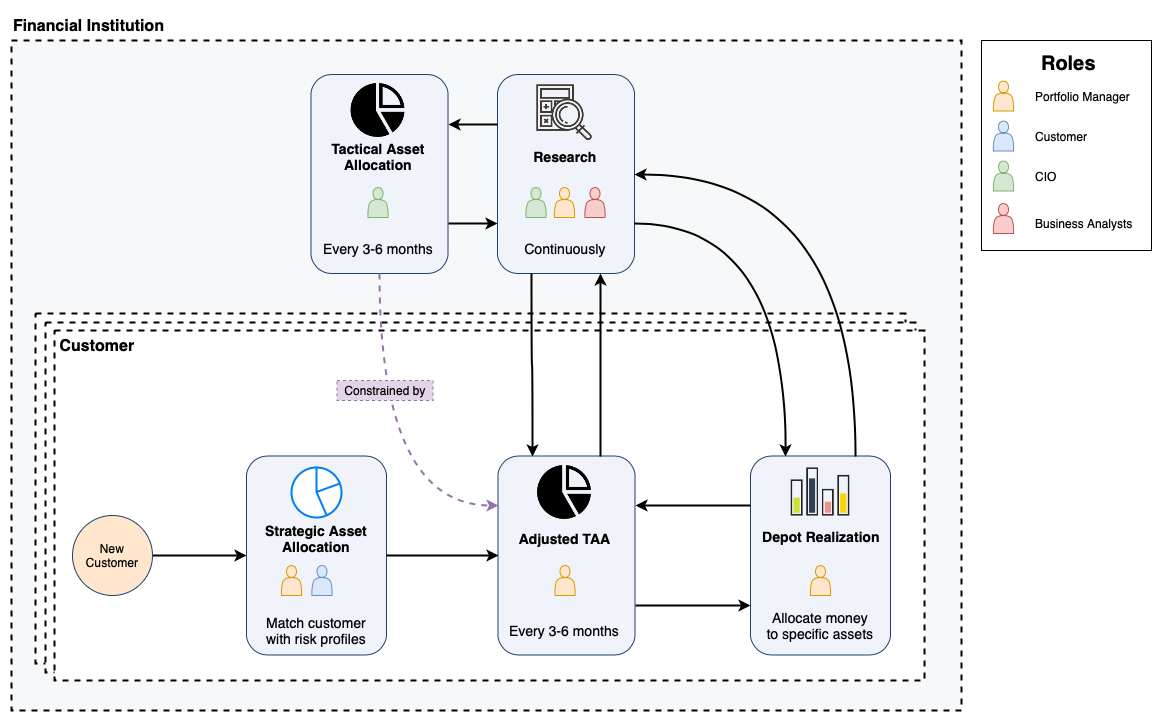
\includegraphics[scale=0.35]{img/work_model_process.png}
  \caption{Work Model of a Professional Portfolio Manager}
  \label{fig:work_model_professional}
\end{figure}


\subsection{Observation of Participants}
Over the course of our project, we were able to attend two real executions of the old portfolio game, during which we observed the teams during their works and spontaneously asked questions where appropriate. The two groups that were observed were quite different, as they had different levels of practical experience:

\begin{itemize}
  \item Participants of the executive education program with current job positions in Banking and Finance related companies, meaning that most participants had some practical experience with the concepts in the game.
  \item Participants of the ``Advanced Portfolio Management Game (S)'' master seminar in the early fall semester, wherein most master students were assumed to possess only theoretical knowledge of the concepts.
\end{itemize}

During the former execution of the game, the simulation itself was played during three days of a seminar. A group of about 30 participants played in groups of three and four. The authors had the chance to observe the groups during their decision-making process and ask them directly for feedback. Additionally, the seminar management collected final feedbacks as well as ideas for further development.\\

This execution of the game was overall very helpful in guiding the initial requirements engineering, as the experienced participants were very clear about their major frustrations with the old application. This lead to many ideas for refinements and features that were incorporated into the user stories and successfully implemented in the new application. Some of the notes compiled during this process can be found in \Cref{sec:appendix_observation_notes}.

For the latter instance of the game, recording software was installed on the computers provided by the DBF, such that all teams could be followed along in their game progress. These recordings were then used to validate the assumptions of user behavior. As the old application required many media breaks (some information was handed out on paper), we were not able to follow these external discussions (without additional sound recordings).


\subsection{Experimental Game with Students}
% TODO: annotated screenshots
Alongside the two executions of the game that we were able to observe, we further managed to set up an experimental setting in cooperation with the DBF team. In this experimental setting, two bachelor-level students with basic knowledge in Finance and two master students with advanced theoretical knowledge of portfolio management played two periods of a supervised game. They were handed out screenshots of the major screens, on which they could annotate everything that came to their mind or that they did not understand. Teams were allowed to ask theoretical questions that were then noted on the corresponding screenshot. The annotated sheets were later converted into a digital aggregation that is appended in \Cref{sec:appendix_observation_notes}. \\

The main goal of this experiment was to gain an understanding of the behavior and problem-solving approaches of players with different levels of experience. This would later allow to tailor the new implementation of the game to these specific needs and to potentially include features that could be activated depending on the level of knowledge of the participants. \\

Over all of the observations with students, a work model from the student perspective was progressively created, refined, and validated. This work model is shown in \Cref{fig:work_model_student}.

\begin{figure}[h!]
  \centering
  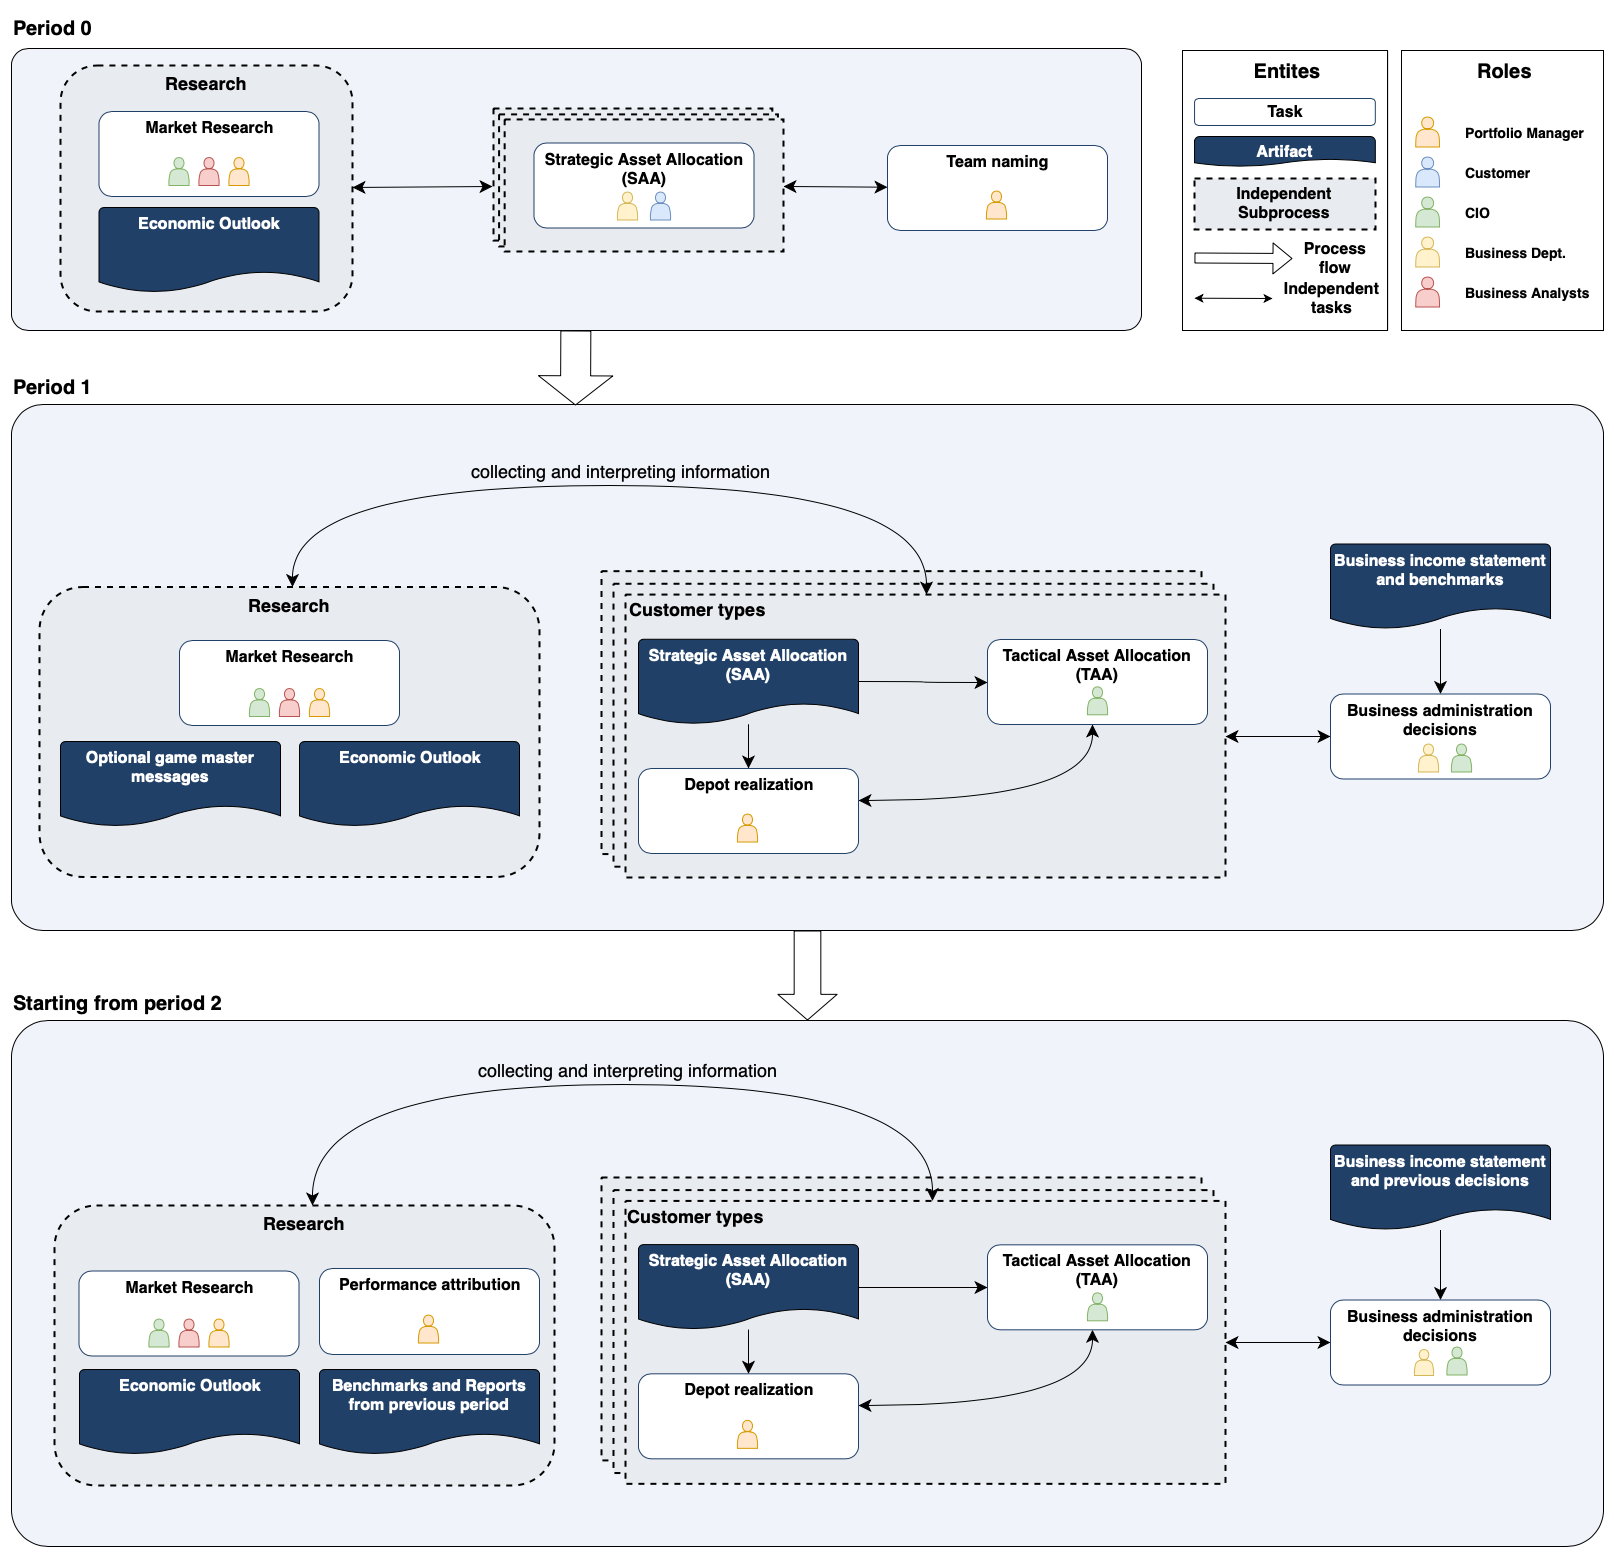
\includegraphics[scale=0.25]{img/work_model_pfm_game.png}
  \caption{Work Model of a Student Participant}
  \label{fig:work_model_student}
\end{figure}




\subsection{Design and Iterative Prototyping}
% TODO: rework
Initially, the authors designed multiple screens based on the predefined work model. Using a sketching software the basic screens for the student's process which includes the SAA, TAA, depot realization and business administration were prototyped. As we realized that the game does not only consist of screens from a student perspective we decided, due to time constraints, to start implementing screens by iterative prototyping. \\

Multiple concepts had to be defined, such as how to model the game session management. By defining a timeline the administrative user always gets a direct response of the state of the game. This colorful timeline builds the base of the game detail screen, while other visualizations or forms within this screen are depending on the state of the game.\\

Another big concept was defining the process of the student's input. The process is depicted on the top located game navigation bar on the right corner. Each processing task (SAA, TAA, depot realization, business administration) has its own progress state. Different concepts have been tried to model this process best intuitive for the users.
% TODO more?
